The lab assignments under-specifies the operation of virtual-indexed caches, as
it does not specify what method to use to avoid aliasing (having multiple
entries in the cache for the same physical address, if it's represented by
multiple virtual addresses).

My implementations do the following when a new block is brought into the cache:
\begin{itemize}
  \item The virtually-indexed physically-tagged cache checks the tags in all
  the cache lines that could potentially hold the virtual address (one line for
  small caches, more lines for large caches), and invalidates any location that
  has the same tag.
  \item The virtually-indexed virtually-tagged cache checks the physical bits
  in the tags (could be zero bits, if the cache is big enough) against the
  physical bits in the new block's address, and invalidates all the blocks
  whose bits match.
\end{itemize}

\section{Question 1}

\section{Question 2}

To determine the working set sizes, I used direct-mapped caches with the
minimum block size (4 bytes). I used a 32Mb cache for computing the compulsory
misses. 32Mb seems like a good size for the RAM in a 2000-era computer, and
higher values made the \texttt{caches} pintool crash.

Figure \ref{q2:miss_rates} shows the miss rates. Table \ref{q2:working_set}
shows the probable working set sizes, based on the miss rates obtained above.

\begin{figure}[htb]
  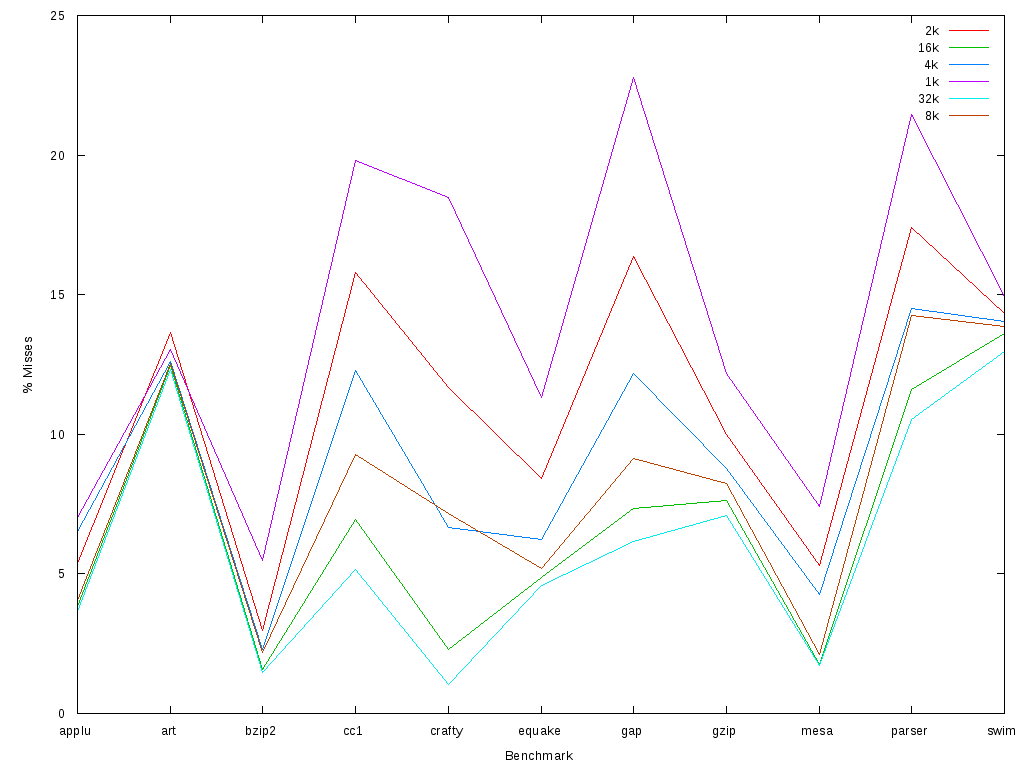
\includegraphics[width=6.8in]{6.823/lab2/figs/working_set.png}
  \caption{Miss rates in direct-mapped physically-indexed physically-tagged
  caches with 4-byte blocks. }
  \label{q2:miss_rates}.
\end{figure}

\begin{figure}[htb]
\center

\begin{tabular}{lcr}
\hline
Benchmark & Integer / FP & Working set size \\
\hline
bzip2 & INT & \\
cc1 & INT & \\
crafty & INT & \\
gap & INT & \\
gzip & INT & \\
parser & INT & \\
\hline
applu & FP & \\
art & FP & \\
equake & FP & \\
mesa & FP & \\
swim & FP & \\
\hline
\end{tabular}

\caption{The working set sizes for the SPEC 2000 benchmark suite. }
\label{q2:working_set}
\end{figure}

\section{Question 3}
The fourth cache model doesn't make any sense. The different cache models in
this lab are motivated by the desire of parallelizing cache access and address
translation.

If the cache is physically indexed, it means the cache access cannot start unil
after address translation. Since we waited for address translation anyway, we
might as well use the physical address for the tag. There's no reason to deal
with the additional complexities of using virtual tagging.

\section{Question 4}
Having more than one process at a time means that each process will have its
own page tables, and therefore the virtual-to-physical mapping can change
during cache operation.

The physically-indexed physically-tagged cache isn't impacted by this change at
all, since it's oblivious to address translation.

The virtually-indexed virtually-tagged cache 

The virtually-indexed physically-tagged cache is equipped to deal with this
change. If the mapping changes, the tag will not match, so the cache will not
give a bad answer by mistake. The cache's design has to deal with aliasing
(different virtual addresses pointing to the same physical address) for the
single-process case, so multiple processes don't introduce a change.

The TAs would have to modify the address translation routine in our source code
to simulate different processes, so I doubt that will be part of the tests. 

\section{Question 5}

I stripped the supplied \texttt{caches} pintool into a pintool that counts the
read and write memory accesses, as well as the aligned reads and writes. The
summaries are presented in figure \ref{q5:unaligned_accesses}.

\begin{figure}[htb]
\center
\begin{tabular}{lrrr}
\hline
Test & \% unaligned reads & \% unaligned writes & \% unaligned accesses \\
\hline
applu & 0.00019\% & 0.00047\% & 0.00023\%  \\
\hline
art & 0.00013\% & 0.00050\% & 0.00019\%  \\
\hline
bzip2 & 0.24491\% & 0.36827\% & 0.28971\%  \\
\hline
cc1 & 0.04994\% & 0.01413\% & 0.03852\%  \\
\hline
crafty & 0.02442\% & 0.01042\% & 0.01913\%  \\
\hline
equake & 0.01114\% & 0.01851\% & 0.01239\%  \\
\hline
gap & 0.08745\% & 0.04416\% & 0.07358\%  \\
\hline
gzip & 0.14022\% & 0.12515\% & 0.13500\%  \\
\hline
mesa & 0.07836\% & 0.08633\% & 0.08100\%  \\
\hline
parser & 0.07013\% & 0.00846\% & 0.04782\%  \\
\hline
swim & 0.00003\% & 0.00007\% & 0.00004\%  \\
\hline
{}Averages & 0.06426\% & 0.06150\% & 0.06342\%  \\
\hline
\end{tabular}

\caption{The percentage of unaligned memory accesses out of the total memory
accesses for the SPEC 2000 benchmark suite. }
\label{q5:unaligned_accesses}
\end{figure}

The bulk of unaligned accesses come from \texttt{bzip2}, which is a
compression tool, and therefore it works with streams of bytes. Other
significant sources of unaligned accesses are also processing streams
of bytes -- \textt{cc} compiles C code, and \textt{parser} presumably builds an
AST out of some language. The one that didn't come to my mind waas
\texttt{mesa}, which is a software OpenGL implementation, and therefore has to
work with a software framebuffer.

The assumption of aligned accesses seems to make sense for most benchmarks. The
numbers reported above are an upper bound of unaligned accesses because, from a
cache perspective, byte accesses can be satisfied even if they're unaligned, and
multibyte accesses are only problematic if they span across 2 cache blocks.
Furthermore, the applications which are most impacted by unaligned access don't
really run on consumer computers -- most people don't compile their code, and a
vast majority of desktop and mobile platforms have accelerated graphics
nowadays.
